\documentclass[10pt]{article}
\usepackage{tikz}
\usetikzlibrary{shapes.misc}
\usepackage[margin=0cm]{geometry}
\pagestyle{empty}
\tikzstyle{every node}=[cross out, draw, red]

\begin{document}

\vspace*{\fill}
\begin{center}
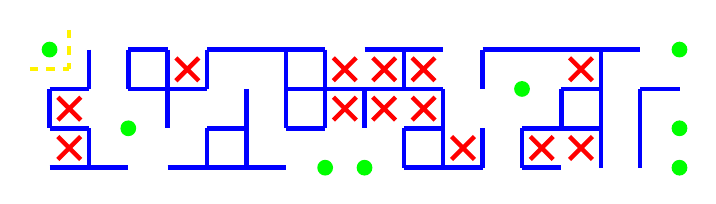
\begin{tikzpicture}[x=0.5cm, y=-0.5cm, ultra thick, blue]
% Walls
    \draw (2,0) -- (3,0);
    \draw (4,0) -- (7,0);
    \draw (8,0) -- (10,0);
    \draw (11,0) -- (15,0);
    \draw (0,1) -- (1,1);
    \draw (2,1) -- (4,1);
    \draw (6,1) -- (10,1);
    \draw (13,1) -- (14,1);
    \draw (15,1) -- (16,1);
    \draw (0,2) -- (1,2);
    \draw (4,2) -- (5,2);
    \draw (6,2) -- (7,2);
    \draw (9,2) -- (10,2);
    \draw (12,2) -- (14,2);
    \draw (0,3) -- (2,3);
    \draw (3,3) -- (6,3);
    \draw (9,3) -- (11,3);
    \draw (12,3) -- (13,3);
    \draw (0,1) -- (0,2);
    \draw (1,0) -- (1,1);
    \draw (1,2) -- (1,3);
    \draw (2,0) -- (2,1);
    \draw (3,0) -- (3,2);
    \draw (4,0) -- (4,1);
    \draw (4,2) -- (4,3);
    \draw (5,1) -- (5,3);
    \draw (6,0) -- (6,2);
    \draw (7,0) -- (7,2);
    \draw (8,1) -- (8,2);
    \draw (9,0) -- (9,1);
    \draw (9,2) -- (9,3);
    \draw (10,1) -- (10,3);
    \draw (11,0) -- (11,1);
    \draw (11,2) -- (11,3);
    \draw (12,2) -- (12,3);
    \draw (13,1) -- (13,2);
    \draw (14,0) -- (14,3);
    \draw (15,1) -- (15,3);
% Pillars
    \fill[green] (0,0) circle(0.2);
    \fill[green] (16,0) circle(0.2);
    \fill[green] (12,1) circle(0.2);
    \fill[green] (2,2) circle(0.2);
    \fill[green] (16,2) circle(0.2);
    \fill[green] (7,3) circle(0.2);
    \fill[green] (8,3) circle(0.2);
    \fill[green] (16,3) circle(0.2);
% Inner points in accessible cul-de-sacs
    \node at (3.5,0.5) {};
    \node at (7.5,0.5) {};
    \node at (8.5,0.5) {};
    \node at (9.5,0.5) {};
    \node at (13.5,0.5) {};
    \node at (0.5,1.5) {};
    \node at (7.5,1.5) {};
    \node at (8.5,1.5) {};
    \node at (9.5,1.5) {};
    \node at (0.5,2.5) {};
    \node at (10.5,2.5) {};
    \node at (12.5,2.5) {};
    \node at (13.5,2.5) {};
% Entry-exit paths without intersections
    \draw[dashed, yellow] (-0.5,0.5) -- (0.5,0.5);
    \draw[dashed, yellow] (0.5,-0.5) -- (0.5,0.5);
\end{tikzpicture}
\end{center}
\vspace*{\fill}

\end{document}
